\subsection{Introduction}
The goal of this text is to give an overview of the geometry behind \'etale cohomology.
\section{Reminder on Schemes}

The basic building blocks of algebraic geometry are affine schemes. An affine scheme $\Spec(A)$ is a geometric object constructed out of the prime spectrum 
\[
  \{p \subseteq A \mid p \text{ prime ideal}\}
\]
of a commutative ring $A$. This set is equipped with the Zariski topology, which has a basis given by sets of the form 
\begin{align*}
  D_f &= \{ p \in \Spec(A) \mid (f) \not \subseteq p \} \\
      &= \{ p \in \Spec(A) \mid f(p) \neq 0\} .
\end{align*}
\begin{definition}
    The \textit{Zariski topology} on $\Spec(R)$ consists of open sets of the form $D_I = \{ p \in \Spec(A) \mid I \not \subset (p)\}$. The closed sets are of the form
    \begin{align*}
        V_I &= \{ p \in \Spec(A) \mid (f) \subseteq p \} \\
            &= \{ p \in \Spec(A) \mid f(p) = 0\},
    \end{align*}
    the \textit{vanishing set} or \textit{zero locus} of $f$. 
\end{definition}

Here $f(p)$ denotes the image of $f$ under the quotient map $A \to A/p$. This notation indicates that we interpret the elements $f \in A$ as functions on the space $\Spec(A)$. Since $f(p) \neq 0$ for all $p \in D_f$, we view the the ring $A[1/f]$ as the ring of rational functions defined on $D_f$. It consists of elements of the form 
\[
  \biggl\{ \frac{g}{f^k} \mid g \in A, k \in \N \biggr\}.
\]
The assingment $D_f \to A[1/f]$ extends to a sheaf $\Sh{O}_{\Spec{A}}: \Spec(A) \to \mathsf{Ring}$, called the \textit{structure sheaf of $\Spec(A)$}. We obtain a fully faithful functor
\[
\Spec : \text{CRing} \to LRS
\]
from the category of commutative rings to the category of locally ringed spaces. An affine schemes is a locally ringed space isomorphic to $\Spec(R)$ for some ring $R$.

\begin{definition}
  A \textit{scheme} is a locally ringed space $X$ such that there is a covering $\{U_i\}_{i \in I}$ of $X$ such that each $U_i$ is isomorphic to an affine scheme $\Spec(A_i)$ for some ring $A_i$.
\end{definition}

\subsection{Motivation for Cohomology}
One of the most important invariants of schemes is \'etale cohomology.  Cohomology is an important invariant in geometry and topology which associates to each space $X$ a sequence of abelian groups $H^i(X)$, $i \ge 0$, the so-called cohomology groups of $X$. For each map $f: X \to Y$ of spaces there are homomorphisms $f^*: H^i(Y) \to H^i(X)$. Moreover there are so called coboundary morphisms $\partial^i : H^i \to H^i+1$ for each $i \ge 0$. In other words, 
\begin{definition}
    a \textit{cohomology theory} for
\end{definition}
We can deduce many interesting properties of spaces from their cohomology groups and the associated homomorphisms.

The first example of cohomology one usually encounters first is singular cohomology. This cohomology theory provides a rigorous way for counting ``holes'' in a topological space.  For instance, the circle $S^1$ has 1 one-dimensional hole while the torus $T^2$ has 2. The sphere $S^2$ has 1 two-dimensional hole but no one-dimensional holes, in symbols 
\footnote{$\Z$ appears here because it is the free group on one generator.}
\begin{align*}
  H^1_{sing}(S^1) \cong \Z,\quad &H^1_{sing}(T^2) \cong \Z \oplus \Z,\\
  H^1_{sing}(S^2) \cong  0,\quad &H^2_{sing}(S^2) \cong \Z.
\end{align*}
One very general approach to cohomology is to use sheaves on a topological space as ``coefficients''. For any space $X$ and any sheaf $\Sh{F}$ on $X$ we can define $H^i(X, \Sh{F})$. Many examples of cohomology turn out to stem from the cohomology of a particular sheaf. For example, if $X$ is a locally contractible space, the singular cohomology $H_{\text{sing}}^i(X)$ of $X$ is isomorphic to the sheaf cohomology $H^i(X, \Z_X)$ of the constant sheaf $\Z_X$ on $X$.

One of the main motivations for \'etale cohomology is that one would like a replacment for singular cohomology for schemes. There are a number of obstacles:
\begin{proposition}\label{scheme_contractible}
    An irreducible scheme is contractible.
\end{proposition}
\begin{proof}
  Define a map $f: X \times I \to X$  by $f(x,0) = x$ and $f(x,t) = \eta$ for $t > 0$. This is a contraction of $X$ onto the point $\eta$, so. the singular cohomology of $X$ is identically 0.
\end{proof}
\begin{proposition}
  $H^i(X, \Sh{F})$ is 0 for any sheaf on an irreducible topological space.
\end{proposition}
\begin{proof}
    See section TODO.
\end{proof}

\subsection{Fundamental groups}
Another important invariant of spaces is the fundamental group. The fundamental group of a pointed topological space $(X,x)$, denoted by $\pi_1(X,x)$ may be defined in two equivalent ways:
\begin{construction}[the fundamental group via paths]
    A loop with base point $x$ is a map $\gamma : [0,1] \to X$ such that $\gamma(0) = \gamma(1) = x$. The homotopy class of $\gamma $ is denoted by $[\gamma]$. Define a composition operation by concatenation: $[\gamma] \circ [\eta] = [\gamma \circ \eta]$, where $\gamma \circ \eta$ is defined to be the path 
    \[\gamma \circ \eta =
        \begin{cases}
            \ \eta(2x) \text{ for } x \in [0, \tfrac{1}{2}]\\
            \ \gamma(2x - 1) \text{ for } x \in [\tfrac{1}{2}, 1].
        \end{cases}
    \]
    It is clear that this construction yields a group structure on the set 
    \[
        \{\ [\gamma] \mid \gamma : [0,1] \to X , \gamma(0) = \gamma(1) = x \}
    \]
    of homotopy classes of loops at $x$.
\end{construction}

\begin{construction}[The fundamental group via covering spaces]
    \begin{definition}
        Let $X$ be a topological space. A \textit{space over $X$ } is a topological space $Y$ together with a continuous map $Y \to X$. A morphis between two spaces $Y_1, Y_2$ over $X$ is a continuous map $f: Y_1 \to Y_2$ such that the diagram
        \[
        % https://q.uiver.app/?q=WzAsMyxbMCwwLCJZXzEiXSxbMiwwLCJZXzEiXSxbMSwxLCJYIl0sWzAsMSwiZiJdLFsxLDIsInBfMiJdLFswLDIsInBfMSIsMl1d
        \begin{tikzcd}
        	{Y_1} && {Y_1} \\
        	& X
        	\arrow["f", from=1-1, to=1-3]
        	\arrow["{p_2}", from=1-3, to=2-2]
        	\arrow["{p_1}"', from=1-1, to=2-2]
        \end{tikzcd}
        \]
        commutes. We obtain the category $\Top/X$ of spaces over $X$.
    \end{definition}
    \begin{definition}
        A space $f: Y \to X$ over $X$ is called a local homeomorphism if for any point $y \in Y$ there is a neighborhood $U$ of $x$ such that the preimage $f^{-1}(U)$ is homeomorphic to a disjoint union of the open sets $f^{-1}(U) \cong \coprod U_i$ such that each $U_i$ gets mapped to $U$ homeomorphically under $f|_{U_i}$. Surjective local homeomorphisms over a space $X$ are also called \textit{covering spaces of $X$} or simply \textit{coverings}.
    \end{definition}
Let $f: Y \to X$ be a surjective local homeomorphism.  A trivial covering is one of the form $p: \coprod X \to X$, where $p$ restricts to the identity on each component. Using this terminology one can also say that a covering is a \textit{locally trivial local homemorphism}. A $Y$-automorphism is defined to be an automorphism of $Y$ in $\Top/X$. 
\begin{definition}
    A covering of $X$ is a \textit{universal covering} if 
\end{definition}
\end{construction}
It requires some work to show that these two notions agree.


\begin{itemize}
  \item  As we have seen in \ref{scheme_contractible}, any irreducible scheme $X$ is contractible. As every loop in an irreducible scheme is contractible, this implies that $\pi_1(X)$ is $0$.
  \item There is no universal covering space.
        For instance, the algebra homomorphism given by $x^n \to x^n, k[x^n] \to k[x]$ corresponds to a map $x \to x^n, \mathbb{A}^1_k \to \mathbb{A}^1_k$. Depicted is the map from $\mathbb{A}^1_\C$ to $\mathbb{A}^1_\C$ for the case $n=2$

          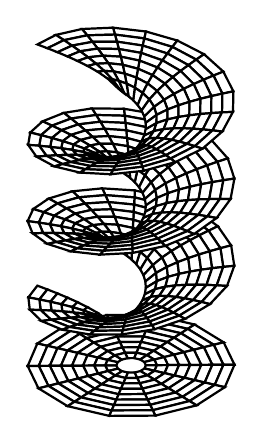
\begin{tikzpicture}[scale=2]
    \begin{axis}[
        axis lines=none,
        axis equal image,
        trig format plots=rad,
        z buffer=sort]
   \addplot3 [
        surf,
        domain=1:7,
        domain y=-pi:pi,
        samples=9,
        samples y=15,
        shader=flat,
        draw=black,
        fill=white
        ]
    ({x*cos(y)},{x*sin(y)},{-12});
   \addplot3 [
        surf,
        domain=1:7,
        samples=9,
        samples y=60,
        shader=flat,
        draw=black,
        fill=white,
        domain y=-3*pi:3*pi
        ]
    ({x*cos(y)},{x*sin(y)},{ln(x)+ y});
    \end{axis}
  \end{tikzpicture}



        This map \textit{should} be local homeomorphism, but this is false in the Zariski topology. There do not exist nonempty open subsets $V$ and $U$ such that $x \to x^n$ maps $V$ isomorphically onto $U$.
  \item fibre bundles aren't locally trivial.
\end{itemize}
  
These issues all stem from the fact that the Zariski topology is very coarse. Grothendieck found a natural generalisation of the notion of topology, allowing not only open subsets $U \subseteq X$ but more generally morphisms of schemes $Y \to X$ to play the role of open set. Specifically, he defined the \textit{\'etale site of $X$}, a generalised topology on $X$, consisting of the following:
\begin{itemize}
  \item The category of \'etale schemes $\text{\'Et}/X$ over $X$. This category consists of schemes $S$ together with an \'etale morphism $f: S \to X$. These morphisms formally behave like local homeomorphisms. 
  \item A notion of covering. In this case a covering of $X$ is a family of \'etale morphisms $\{\varphi_i: U_i \to X\}$ such that they are jointly surjective, $\bigcup_i im(\varphi_i) = X$. We will make this more precise later.
\end{itemize}
It will turn out that surjective \'etale maps are the right notion for a good covering theory for schemes. In particular they will allow us to define fundamental groups. Furthermore, the \'etale site will fix the issues we had in defining cohomology as well.

The \'etale topos $\mathsf{Sh}(X)$ of a scheme $X$ is the category of sheaves on the \'etale site of $X$.  The \'etale topos $\mathsf{Sh}(X)$ may be thought of as a generalised space, locally modeled on $X$, with a close relation to the geometric properties of $X$. 

Because \'etale morphisms behave like local homeomorphisms, it is possible to realise the theory of covering spaces for schemes. In particular this means that we get a good notion the fundamental groups $\pi_1(X)$. Furthermore, the \'etale topos $\mathsf{Sh}(X)$ also allows us to compute cohomology for sheaves which have vanishing cohomology in the Zariski setting. In this sense the \'etale site of a scheme is a much finer topology than the Zariski topology.


\subsection{Interpretation of Cohomology}
Cohomology groups are not just of interest in their own right. In many cases, one can show that the cohomology classes $[\gamma] \in H^n(X, \Sh{A})$ correspond bijectively to some other kind of geometrical construction involving $X$.

For instance, when $p:Z \to B$ is a map of topological spaces and $\Sh{G}$  is a sheaf of subgroups of $Aut_B(Z)$, one can define a notion of “twist of $p$ with structure sheaf $\Sh{G}$”. One obtains the bijection
\begin{align}
            \left\{ \parbox[c]{1.1in}{\centering
                       Isomorphism classes of twists of $p$
                       with structure sheaf $\Sh{G}$}
            \right\}
            \stackrel{\sim}{\to}
            \parbox[c]{0.5in}{\centering
                       $H^1(B, \Sh{G})$}
\end{align}

There is also a bijection
\begin{align}
            \left\{ \parbox[c]{1.1in}{\centering
              Isomorphism classes of vector bundles of rank $n$ with basis $B$}
            \right\}
            \stackrel{\sim}{\to}
            \parbox[c]{0.5in}{\centering
            $H^1(B, GL_{n,B})$}
\end{align}
and in particular
\begin{align}
            \left\{ \parbox[c]{1.1in}{\centering
            Isomorphism classes of line bundles with basis $B$}
            \right\}
            \stackrel{\sim}{\to}
            \parbox[c]{0.5in}{\centering
                $H^1(B, \Ring(O)_B^\times)$}
\end{align}

\subimport{introduction/}{mobius.tex}
\section{prerequisites}
We assume aqcuaintance with the basics of category theory including limits and adjoint functors. We will make free use of results from algebra but will provide references wherever needed. We will also use basic notions of scheme theory.